%\VignetteIndexEntry{CoRegNet visualization examples}
%\VignetteKeyword{Network}
%\VignettePackage{CoRegNet}
\documentclass[12pt]{article}

\textwidth=6.2in
\textheight=8.5in
\oddsidemargin=0.2in
\evensidemargin=0.2in
\headheight=0in
\headsep=0in

\usepackage{Sweave}
\begin{document}
\Sconcordance{concordance:CoRegNetExamples.tex:CoRegNetExamples.Rnw:%
1 12 1 1 0 69 1}


\title{CoRegNet visualization examples}
\author{R\'emy Nicolle, Thibault Venzac, Mohamed Elati}
\date{10 October 2014}
\maketitle

This vignette contains snapshots of the shiny interactive user interface for the visualization of a co-regulatory network driving  bladder cancer.


The Co-regulation page is divided in three parts (see figure \ref{fig:webpage}).
In the top left corner, a control panel lists the samples and samples subtype to analyze, the number of minimum GRN to select significant cooperative interactions and an input to search for a particular TF in the network.
In the right part, an interactive Cytoscape javascript widget display the network of co-regulators. The color of the nodes reflects the activity of the TF in the selected subtype as shown in figure \ref{fig:subtypeCoreg} for two types of bladder cancers.
The bottom part of the page contains a plot reactive to action performs on the network.



\begin{figure}
\caption{View of the shiny Web page.}
\label{fig:webpage}
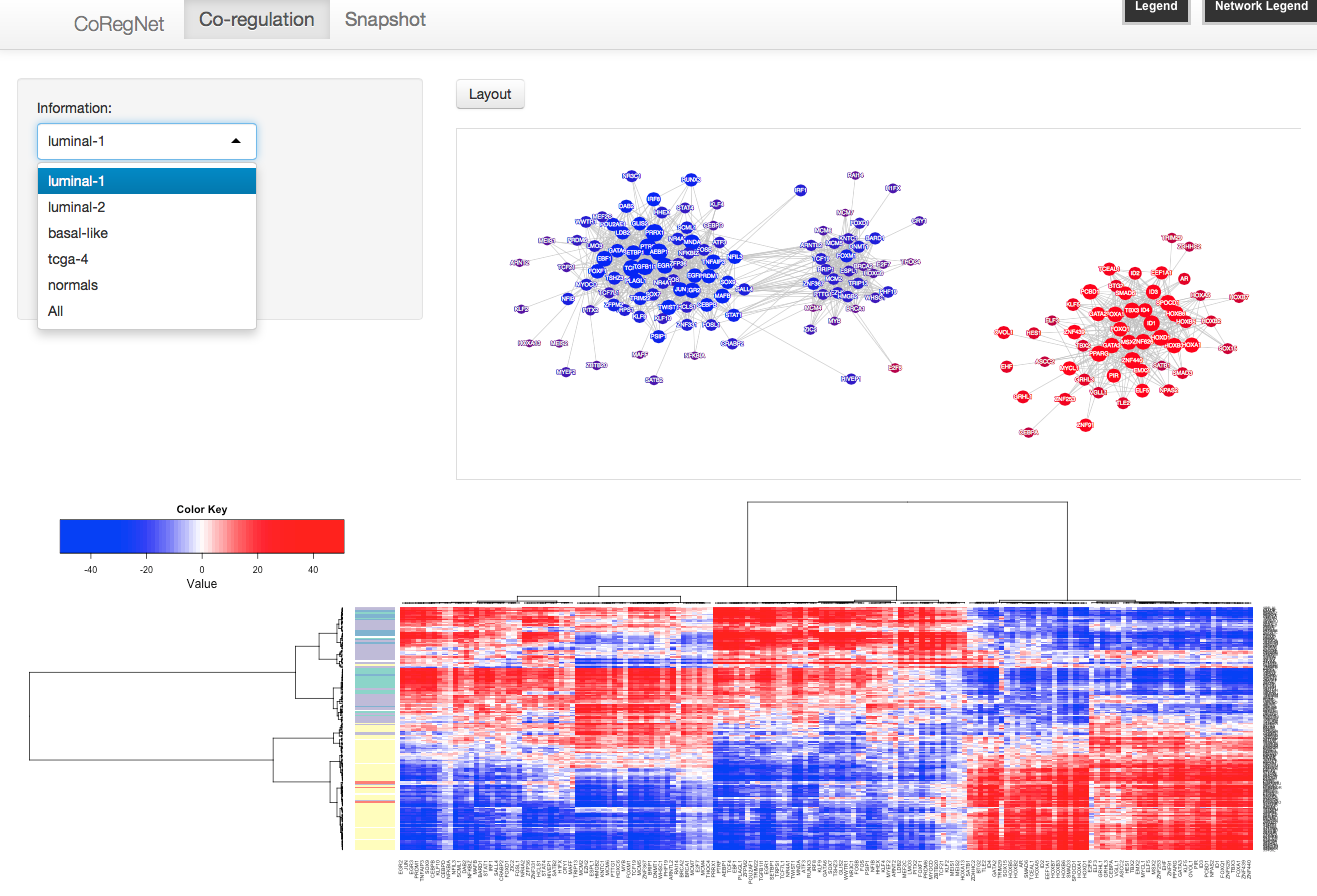
\includegraphics{fig/wholeApp}
\end{figure}

\newpage


\begin{figure}[hp!]
\centering
{\LARGE Basal-like bladder cancer co-regulator network}
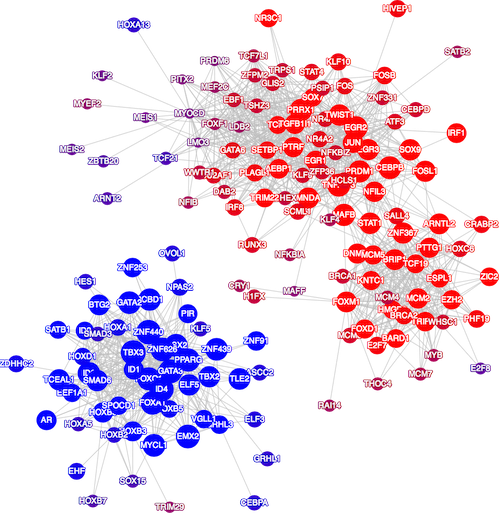
\includegraphics[width=0.7\linewidth]{fig/basal1}
\\
{\LARGE Luminal-like bladder cancer co-regulator network}
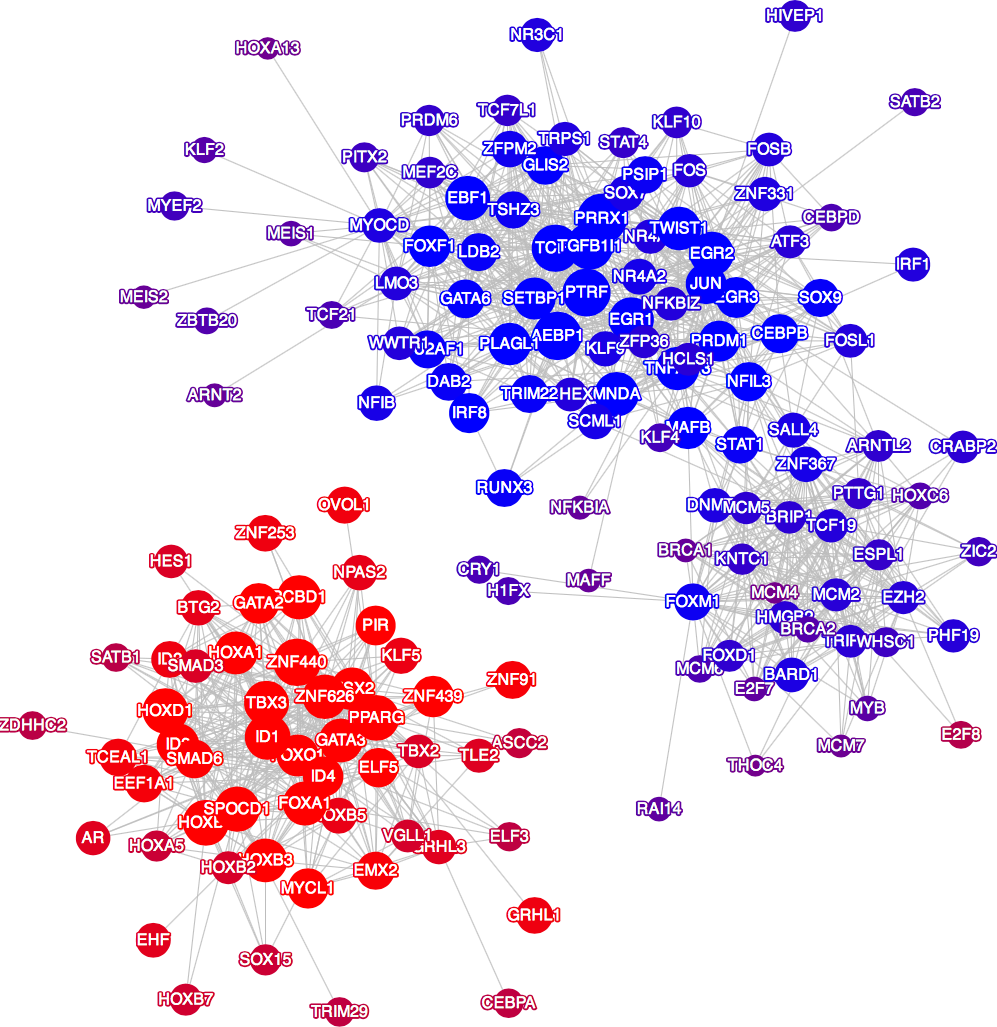
\includegraphics[width=0.7\linewidth]{fig/luminal1}
\caption{Subtype specific co-regulator network. The color of each TF/node is based on the mean influence in all samples of the subtype.}
\label{fig:subtypeCoreg}
\end{figure}

\newpage

When no nodes are selected in the Cytoscape widget, a heatmap of the TF influence is displayed. When several nodes are selected, the heatmap will contain only the influence of the selected TF.
The selection of a single TF will display a multi-layer heatmap for each type of information given as an input to the application.
An example is shown in figure \ref{fig:PPARGLocalView}.
The first heatmap color codes the sample classification. The second shows the Copy Number status of the select TF. The third and fourth show the influence and expression values of the selected TF. Finally, the fifth and sixth heatmap display the expression of the activated and repressed genes respectively.



\begin{figure}[h!]
\centering
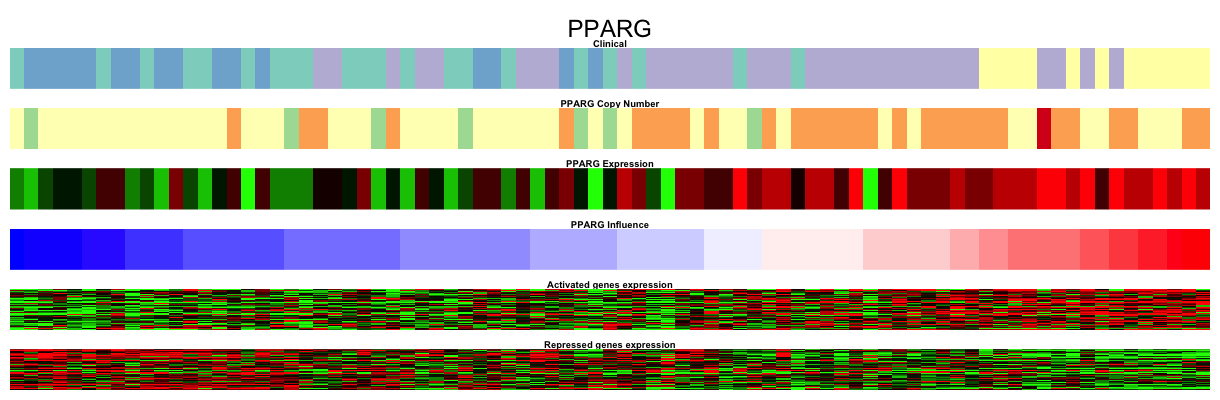
\includegraphics[width=0.7\linewidth]{fig/PPARGLocalView}
\caption{Local TF related heatmap.
Expression is color coded from green to red (low to high) and the influence from blue to red (low to high). Heatmaps display one sample per column.
}
\label{fig:PPARGLocalView}
\end{figure}

\newpage

Finally, when additional regulatory evidences were integrated in the network, the Cytoscape network will display these interactions in addition to the inferred co-regulation interactions as shown in figure \ref{fig:coregnetWithEvidence}. Regulatory evidences will be displayed as directed edges between TF while cooperative evidences will be shown as undirected edges.

\begin{figure}[h!]
\centering
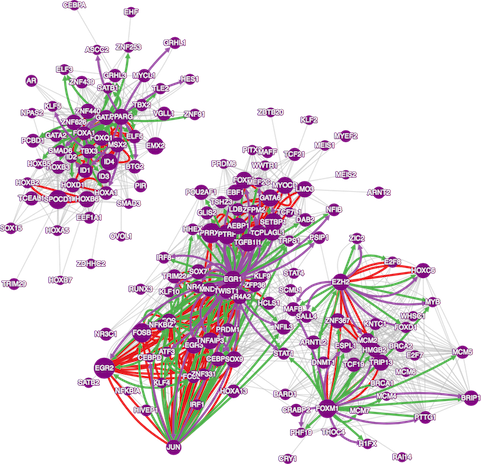
\includegraphics[width=0.5\linewidth]{fig/coregnetWithEvidence}
\caption{Multiple type of interactions. Grey : predicted cooperative interactions. Green : regulatory interactions from the ENCODE ChIP-seq data. Purple : regulatory interactions from the CHEA2 ChIP data. Red : protein interaction from the STRING database. }
\label{fig:coregnetWithEvidence}
\end{figure}


\end{document}

